\clearpage
\pagestyle{fancy}
\fancyhf{}
\fancyhead[R]{\thepage}
\phantomsection% 
\addcontentsline{toc}{chapter}{LEMBAR PENGESAHAN}

\begin{center}

	\large \bfseries \MakeUppercase{Lembar Pengesahan}
    
    \small \normalfont \singlespacing \justify{
    Saya menyatakan bahwa Tugas Akhir berjudul “{\thetitle}" merupakan hasil karya saya sendiri dan belum pernah diajukan, baik sebagian maupun seluruhnya, di Institut Teknologi Sumatera atau institusi pendidikan lain oleh saya maupun pihak lain.}
    %Tugas Akhir Sarjana dengan judul "{\thetitle}" adalah benar dibuat oleh saya sendiri dan belum pernah dibuat dan diserahkan sebelumnya, baik sebagian ataupun seluruhnya, baik oleh saya ataupun orang lain, baik di Institut Teknologi Sumatera maupun di institusi pendidikan lainnya.

	% Informasi Mahasiswa
    \flushleft
	\setlength{\tabcolsep}{0pt}
	\begin{tabular}{p{0.59\textwidth} p{0.3\textwidth}}
        \vspace{0.1cm}
		Lampung Selatan, \today & %
		\multirow{6}{*}{
			% Kotak pasfoto 3x4
			\phantom{----------------------} % Amazing hack biar kotaknya ke kanan (RDB)
			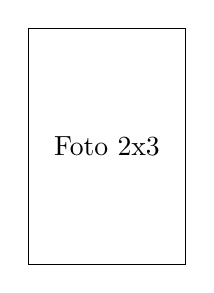
\begin{tikzpicture}
				\draw rectangle (2cm,3cm) node[pos=0.5] {Foto 2x3};
			\end{tikzpicture}
		}\\
		Penulis, \\
		& \\
		& \\
		%& \\
		\theauthor\\
		NIM. \printnim
	\end{tabular}
	% Informasi Dosen
	\vspace{0.4cm}
        \begin{center}
        Diperiksa dan disetujui oleh,
        \end{center}
        \vspace{0.1cm}

	\justify
    \setlength{\tabcolsep}{0pt}
    \begin{tabular}{ m{0.5cm}  m{0.7\textwidth} >{\centering\arraybackslash}m{0.3\textwidth}}
        \multicolumn{2}{c}{\hspace*{70pt}Pembimbing} & \multicolumn{1}{c}{} \\[2pt]
		1. & \printnamadosbinga & \\
		 & \printnipdosbinga & ............... \\%[4pt]
		 & \\
		2. & \printnamadosbinga & \\
		& \printnipdosbinga & ............... \\%[4pt]
		& \\
		\multicolumn{2}{c}{\hspace*{70pt}Penguji} & \multicolumn{1}{c}{} \\[2pt]
		1. & \printnamapengujia & \\
		& \printnippengujia & ............... \\[4pt]
            %& \\
		2. & \printnamapengujib & \\
		& \printnippengujib & ............... \\
    \end{tabular}
%	\vfill

	\begin{center}
		\fontsize{10pt}{10pt}
        \vspace{0.45cm}
		Disahkan oleh,\\
		Koordinator Program Studi Teknik Informatika\\
		Fakultas Teknologi Industri\\
		Institut Teknologi Sumatera
		\vspace{1.8cm}\\
		Andika Setiawan, S.Kom., M.Cs. \\ % TODO: make automatic
		NIP. 19911127 2022 03 1 007 \\
	\end{center}
	\vfill

\end{center}
\clearpage